%-----------------------------------------------------------------------------------
%	PACKAGES AND OTHER DOCUMENT CONFIGURATIONS
%----------------------------------------------------------------------------------



\documentclass[11pt]{article}

\usepackage[top=2cm, bottom=3cm, left=2cm, right=2cm]{geometry}

\setlength{\parindent}{0in}

\newcommand{\Var}{\mathrm{Var}}

\newcommand{\Cov}{\mathrm{Cov}}

\newcommand{\plim}{\rightarrow_{p}}

\usepackage{amsmath, amsfonts}
\usepackage{graphicx}
\usepackage{pdfpages}
\usepackage{bm}
\usepackage{listings}

% Expectation symbol
\newcommand{\E}{\mathrm{E}}
\newcommand{\V}{\mathrm{V}}
\newcommand{\N}{\mathcal{N}}

%----------------------------------------------------------------------------------
%	TITLE AND AUTHOR(S)
%----------------------------------------------------------------------------------

\title{Econ 621 Assignment 5} % The article title


\author{Nathan Mather} % The article author(s) 

\date{\today} % An optional date to appear under the author(s)

%----------------------------------------------------------------------------------
\begin{document}
	
%------------------------------------------------------------------------------
%	TABLE OF CONTENTS & LISTS OF FIGURES AND TABLES
%------------------------------------------------------------------------------
\maketitle % Print the title/author/date block

\setcounter{tocdepth}{2} % Set the depth of the table of contents to show sections and subsections only




%----------------------------------------------------
% Question 1
%---------------------------------------------------- 
\section{Question 1}

(2) and (3) differ because (2) is an elasticity holding utility constant. This means that as my wage changes I am compensated in some way so that my total utility is unchanged. However, it is possible to have the same total utility but have different marginal utility of wealth. For example, If my wage falls and I am compensated by more free time it is possible that my utility would remain the same, but my marginal utility of wealth is higher because I have less money. This would change the marginal benefit of working an additional hour and receiving the wage W. (3) holds the actual marginal utility of wealth constant as I change the wage, meaning that the marginal benefit of working another hour and receiving W more dollars has not changed. \\

Intuitively (3) would be bigger because Under (2) as my wage increases my wealth increases and lowers the marginal utility of an extra dollar. So I wont change my behavior as much as if that marginal utility per dollar was fixed . \\

In MaCurdy's model we have 
$$ \eta = \delta+\gamma(t) < \eta |_u = \delta + \gamma(t) -E(t) \theta < \eta|_{\lambda} = \delta
$$

Where $\delta$ is the intertemporal substitution elasticity, 



%----------------------------------------------------
% Question 2
%---------------------------------------------------- 
\section{Question 2}

\pagebreak

%----------------------------------------------------
% Question 3
%---------------------------------------------------- 
\section{Question 3}
\subsection{a}
The estimate for $\delta$ is -.339 This is surprising as I would expect that as wages increase most people would work more and not less. Although, because of income effects it is possible to have a backwards bending labor supply curve. 
\\ \\ 

On the other hand there is division bias in the wage variable biasing the result towards -1. So in some sense it is not surprising. Additionally wages are endogenous. The arrival of new information affects not only the wage rates, but also leads to a revision in expected lifetime wealth which also biases the result downwards. 

\subsection{b}
The estimate for $\delta$ is now .1233444 The result is positive, which is supported by theory. However, the confidence interval includes zero. 

\subsection{c}
 They are jointly significant with an F test of  2.8. While the coefficients are jointly significant this is below the rule of thumb benchmarks of 10 or 20 and so these instruments should be considered weak sauce. This suggests the results are significantly biased. 

 
 \subsection{d}
 under liml $\delta = .5090904  $. This is positive and higher than the estimate in part b. I expected this as liml performs better under weak instruments than 2sls.
 
 \subsection{e}
 The standard 2sls CI is $ [-.165132,    .4118207]$. The Confidence interval based on Moreira's CLR test is $[    -.23,    1.59]$ while the Anderson-Rubin condence interval is $ [    -.21,    1.15] $. These confidence intervals are much larger. This is what we would expect as the weak instruments are leading to SE that are too small. 
  
  \subsection{f}
  He does this because many of the 14 instruments are incredibly weak and dropping some of them may actually increase the joint F test of the variables. We see that it, in fact, does.  
  
  \subsection{g}
  The joint f test for these 5 variables is  $5.33$. This is better than with all 14 but should still be considered weak. 
  
  \subsection{h}
  $\delta = .2903494  $ which is higher than with 14 instruments, as expected. Adding additional weak instruments only biases the result towards OLS which is biased downwards in this case. 
  
  \subsection{i}
  $\delta = .4157539  $ which is similar to what we found before. This is to be expected as LIML is median unbiased so the estimate should not change much. 
  
  \subsection{j}
  The confidence interval is $ [    -.07,    1.28]$. This is more precise than when using 14 instruments, as expected. The 5 instruments had a higher F test than all 14 and so are less weak sauce. 
  
   \subsection{k}
  The full sample estimate gives $\delta =  -.257353  $ which is comparable to before. 
  
  \subsection{l}
  The f test is not 7.53. This is significantly higher than before, but still below even a low general cutoff of 10. 
  
  \subsection{m}
  The 2sls estimate is .2602845  while the liml is .355197 THe 2sls estimate has increase by  lot compared to the limited sample and the liml has not changed much. As expected since 2sls is more affected by weak instruments. 
  
  \subsection{n}
  The confidence interval is $  [     .12,      .6]$ Which is much more precise than with the smaller sample. 
  
  \subsection{o}
  the 2sls estimate is .2777046  while the liml is  .3330571. Both are comparable to what we found before.
  
  \subsection{p}
  
  The confidence interval is $[      .1,     .53]$ which is much smaller than with the small sample and a bit smaller than with the large sample and 14 instruments.
  
  
  \subsection{STATA Code}
  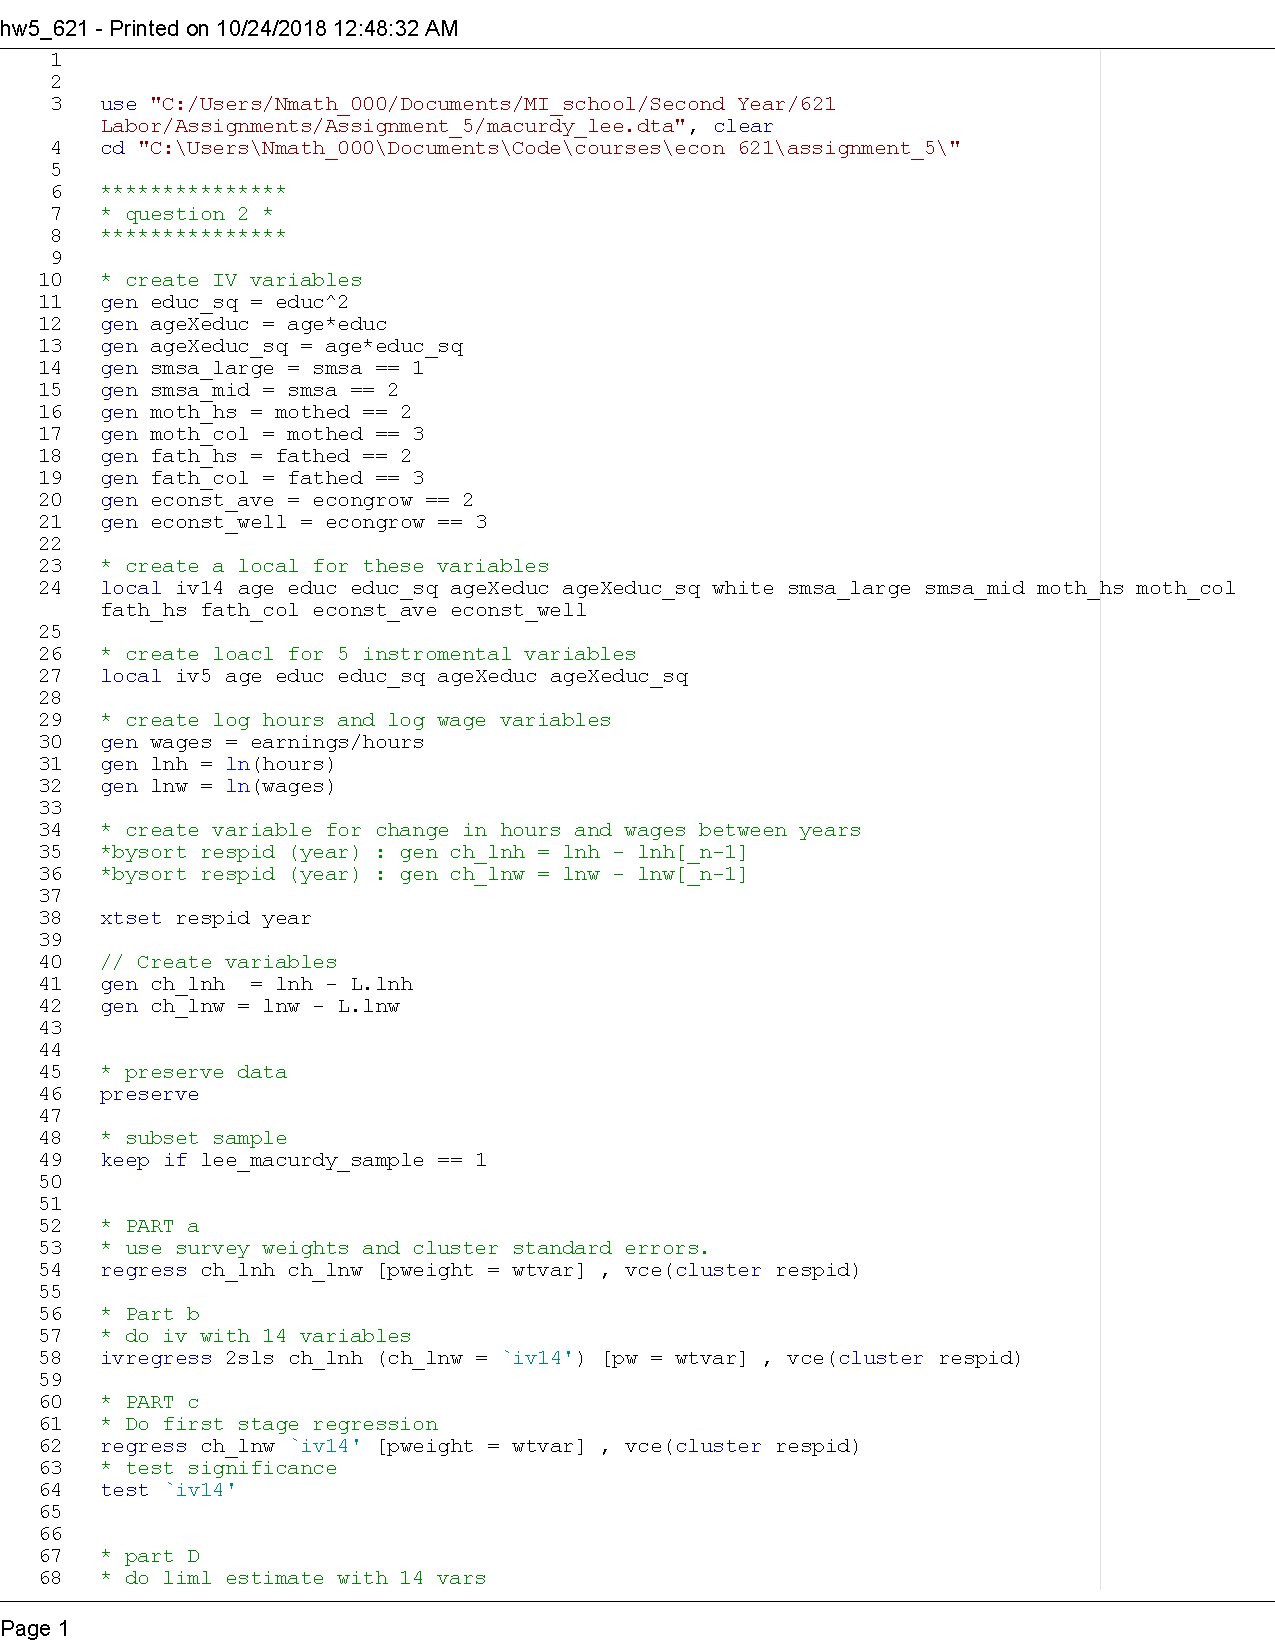
\includepdf[page=-]{code_621_ps5.pdf}
  
 
  
 %------------------------------------------------
% end doc
%------------------------------------------------
\end{document}


